\begin{figure}[ht]\centering
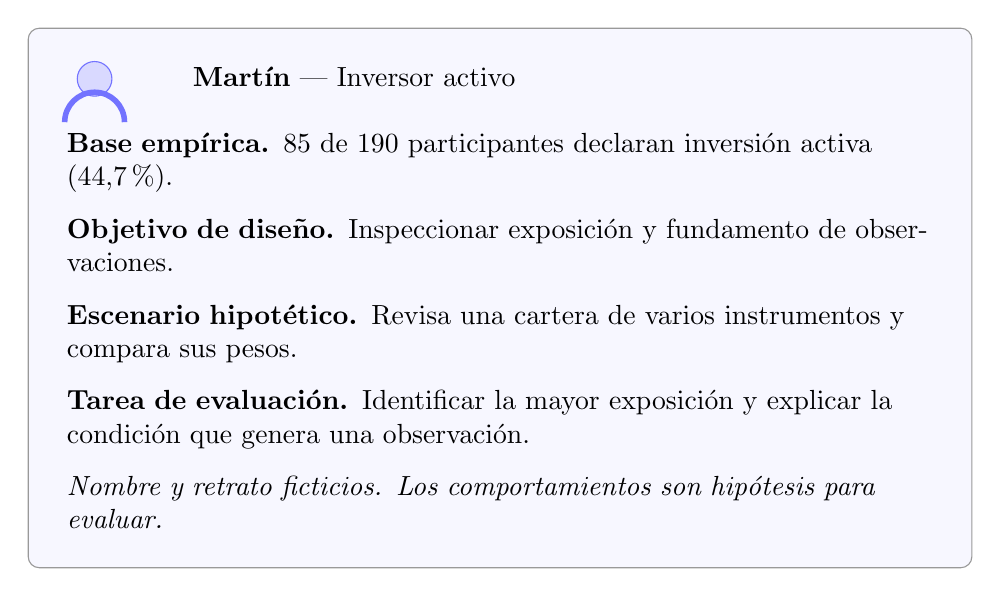
\begin{tikzpicture}
\node[draw=black!40,rounded corners,fill=blue!3,text width=11cm,inner sep=14pt,align=left] (card) {\hspace{1.6cm}\textbf{Martín} --- Inversor activo\\[12pt]
\textbf{Base empírica.} 85 de 190 participantes declaran inversión activa (44,7\,\%).\\[7pt]
\textbf{Objetivo de diseño.} Inspeccionar exposición y fundamento de observaciones.\\[7pt]
\textbf{Escenario hipotético.} Revisa una cartera de varios instrumentos y compara sus pesos.\\[7pt]
\textbf{Tarea de evaluación.} Identificar la mayor exposición y explicar la condición que genera una observación.\\[7pt]
\textit{Nombre y retrato ficticios. Los comportamientos son hipótesis para evaluar.}};
\begin{scope}[shift={([xshift=0.85cm,yshift=-0.65cm]card.north west)}]
\draw[fill=blue!15,draw=blue!55] (0,0) circle (0.22);
\draw[draw=blue!55,line width=2pt] (-0.38,-0.55) arc[start angle=180,end angle=0,radius=0.38];
\end{scope}
\end{tikzpicture}
\caption{Persona usuaria: inversor activo. Fuente: elaboración propia.}\label{fig:persona-activo}
\end{figure}

\begin{figure}[ht]\centering
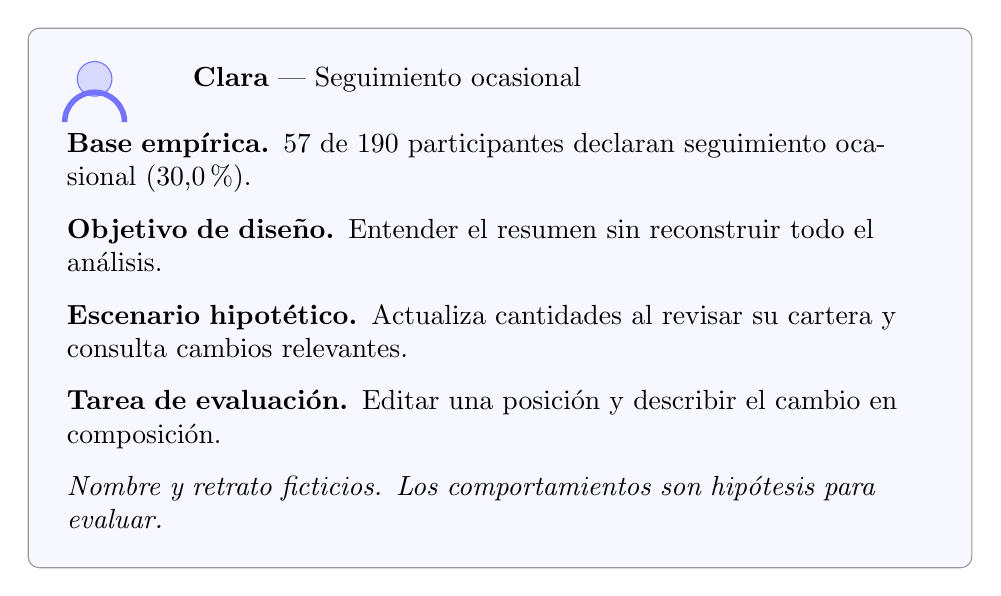
\begin{tikzpicture}
\node[draw=black!40,rounded corners,fill=blue!3,text width=11cm,inner sep=14pt,align=left] (card) {\hspace{1.6cm}\textbf{Clara} --- Seguimiento ocasional\\[12pt]
\textbf{Base empírica.} 57 de 190 participantes declaran seguimiento ocasional (30,0\,\%).\\[7pt]
\textbf{Objetivo de diseño.} Entender el resumen sin reconstruir todo el análisis.\\[7pt]
\textbf{Escenario hipotético.} Actualiza cantidades al revisar su cartera y consulta cambios relevantes.\\[7pt]
\textbf{Tarea de evaluación.} Editar una posición y describir el cambio en composición.\\[7pt]
\textit{Nombre y retrato ficticios. Los comportamientos son hipótesis para evaluar.}};
\begin{scope}[shift={([xshift=0.85cm,yshift=-0.65cm]card.north west)}]
\draw[fill=blue!15,draw=blue!55] (0,0) circle (0.22);
\draw[draw=blue!55,line width=2pt] (-0.38,-0.55) arc[start angle=180,end angle=0,radius=0.38];
\end{scope}
\end{tikzpicture}
\caption{Persona usuaria: seguimiento ocasional. Fuente: elaboración propia.}\label{fig:persona-ocasional}
\end{figure}

\begin{figure}[ht]\centering
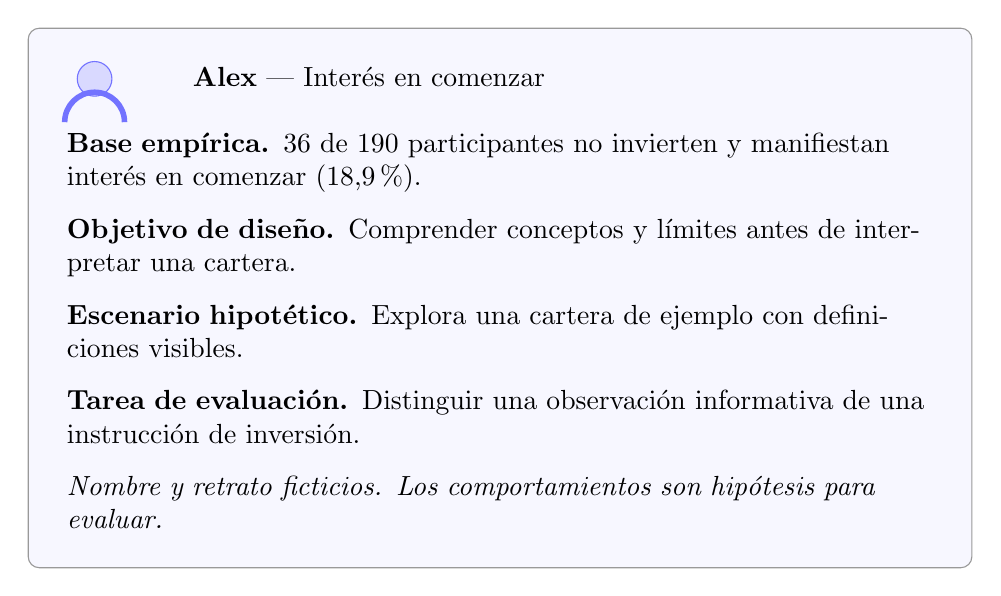
\begin{tikzpicture}
\node[draw=black!40,rounded corners,fill=blue!3,text width=11cm,inner sep=14pt,align=left] (card) {\hspace{1.6cm}\textbf{Alex} --- Interés en comenzar\\[12pt]
\textbf{Base empírica.} 36 de 190 participantes no invierten y manifiestan interés en comenzar (18,9\,\%).\\[7pt]
\textbf{Objetivo de diseño.} Comprender conceptos y límites antes de interpretar una cartera.\\[7pt]
\textbf{Escenario hipotético.} Explora una cartera de ejemplo con definiciones visibles.\\[7pt]
\textbf{Tarea de evaluación.} Distinguir una observación informativa de una instrucción de inversión.\\[7pt]
\textit{Nombre y retrato ficticios. Los comportamientos son hipótesis para evaluar.}};
\begin{scope}[shift={([xshift=0.85cm,yshift=-0.65cm]card.north west)}]
\draw[fill=blue!15,draw=blue!55] (0,0) circle (0.22);
\draw[draw=blue!55,line width=2pt] (-0.38,-0.55) arc[start angle=180,end angle=0,radius=0.38];
\end{scope}
\end{tikzpicture}
\caption{Persona usuaria: interés en comenzar. Fuente: elaboración propia.}\label{fig:persona-principiante}
\end{figure}
